\section{Equazione del bilancio energetico}\label{sec:bilancio-energetico}
L'\emph{equazione del bilancio energetico} esprime l'energia che emerge da ogni \emph{shell} della struttura stellare, essenzialmente dovuta alle reazioni termonucleari. Si può scrivere:
\begin{equation}\label{eq:bilancio-energetico}
    \dfrac{\ud L(r)}{\ud r} = 4 \pi r^2 \rho(r) \epsilon
\end{equation}
dove $L(r)$ è la luminosità emergente dalla sfera di raggio $r$ e $\epsilon$ l'energia prodotta da ogni shell per unità di tempo e di massa, $[\epsilon] = \si{erg.s^{-1}.g^{-1}}$.

\subsection{Ricavare l'equazione}
È semplice ricavare tale equazione. consideriamo, infatti, l'usuale guscio di gas a una distanza $r$ dal centro.. Sia $L(r)$ la luminosità emergente dalla porzione di stella delimitata dal guscio a raggio $r$ e analogamente per $L(r + \ud r)$. Possiamo scrivere:
\[
L(r + \ud r) - L(r) = \ud L(r) = 4 \pi \rho r^2 \ud r \epsilon
\]
dove $4 \pi \rho r^2 \ud r$ rappresenta la massa del guscio di sfera tra $r$ e $r + \ud r$ e $\epsilon$ è l'energia prodotta da ogni guscio per unità di tempo e di massa. Attenzione, \emph{non} si tratta dell'energia radiata dalla stella. In questo modo si riottiene la definizione di luminosità (par.~\ref{sec:luminosità}).

Consideriamo un tipico profilo di luminosità radiale per una stella (fig.~\ref{fig:profilo-luminosità-sole}): la luminosità varia con $r$ sono in una regione ristretta della stella, corrispondente al suo centro, poi verso l'esterno diventa costante. All'esterno, secondo la eq.~\eqref{eq:bilancio-energetico} vale $\epsilon = 0$ e questo ci dice che tutta l'energia viene prodotta nelle regioni interne, come ci aspettiamo dal fatto che le reazioni termonucleari hanno bisogno di una elevata temperatura per poter avvenire. Tuttavia, le reazioni termonucleari \emph{non} sono le uniche a poter contribuire all'energia, in particolare anche la \emph{contrazione gravitazionale} può produrre energia, e tale contributo non è incluso nell'eq.~\eqref{eq:bilancio-energetico}. Per capire come la contrazione gravitazionale possa contribuire all'energia, bisogna far riferimento al \emph{teorema del viriale}.

\begin{figure}
\centering
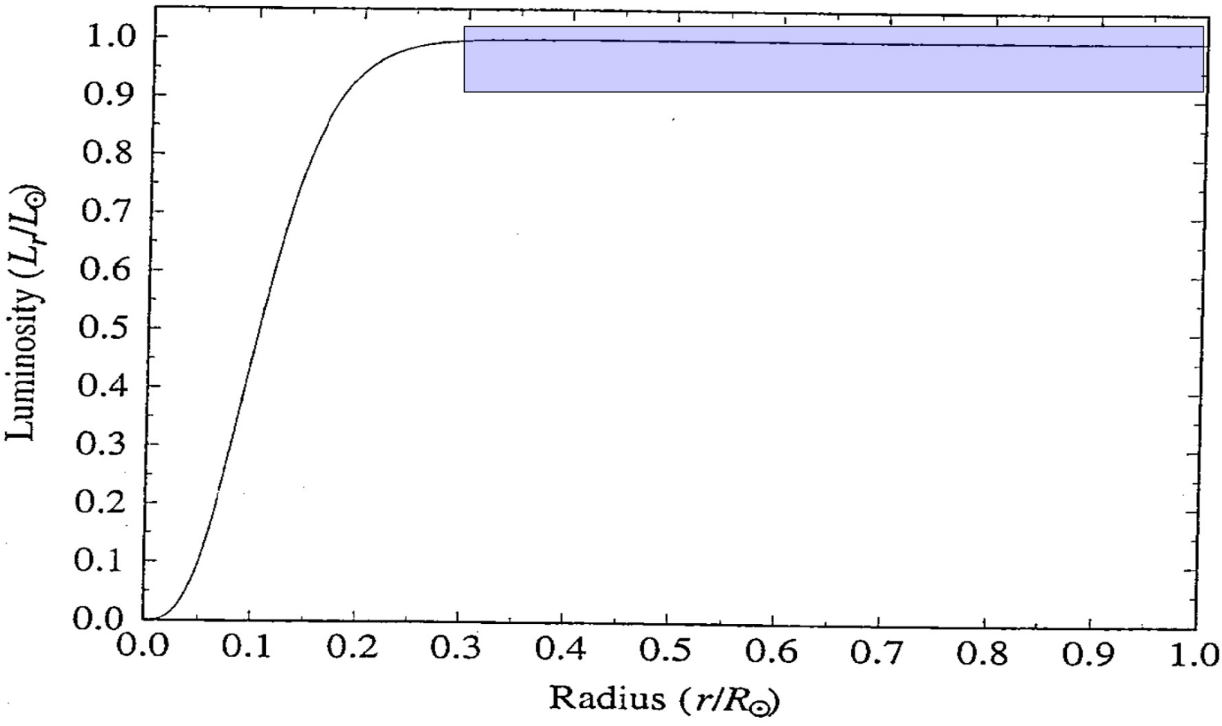
\includegraphics[width=0.5\textwidth]{immagini/profilo-luminosita-radiale-sole.png}
\caption{Profilo di luminosità radiale del Sole. Nella zona evidenziata si ha $L(r) = \textup{const}$, da cui, secondo eq.~\eqref{eq:bilancio-energetico}, $\epsilon = 0$. Questo ci dice che negli strati esterni della stella non viene prodotta energia e le reazioni termonucleari sono concentrate nell'interno stellare, dove infatti le temperature sono più elevate.}
\label{fig:profilo-luminosità-sole}
\end{figure}

\subsection{Teorema del viriale}
Per ogni sistema in equilibrio di particelle auto-gravitanti, come nel caso delle strutture stellari, vale il \emph{teorema del viriale}:
\begin{equation}\label{eq:teorema-viriale}
    2K + \Omega = 0
\end{equation}
dove $K$ è l'energia cinetica del sistema e $\Omega$ l'energia potenziale. L'eq.~\eqref{eq:teorema-viriale} dice sostanzialmente che a una contrazione ($\ud \Omega < 0$) segue un aumento dell'energia cinetica, e quindi un aumento della temperatura. Scrivendo inoltre l'energia totale del sistema come $U = K + \Omega$, si ha
\[
U = - \frac{\Omega}{2} + \Omega \implies U = \frac{\Omega}{2}
\]
ovvero a una contrazione ($\ud \Omega = 0$) segue una diminuzione dell'energia totale del sistema ($\ud U < 0$).

Le due relazioni considerate precedentemente:
\begin{equation}\label{eq:viriale-differenziale}
\ud U = \frac{\ud \Omega}{2} \qquad \ud K = - \frac{\ud \Omega}{2}
\end{equation}
mostrano che in ogni contrazione ($\ud \Omega$) \emph{metà} dell'energia è \emph{emessa} e \emph{metà} dell'energia è usata per incrementare la temperatura del caso. Possiamo riformulare quanto detto in un altro modo: ogni perdita di energia totale $\ud U$ dovuta a emissioni genera una contrazione del sistema, che produce anche un incremento della temperatura interna.

Come stimare il contributo della contrazione gravitazionale alla luminosità di una stella? Se fosse elevato andrebbe corretta l'eq.~\eqref{eq:bilancio-energetico}. Per capirlo utilizziamo la~\eqref{eq:viriale-differenziale} per scrivere
\[
L = \frac{\ud U}{\ud t} = \frac{1}{2} \abs*{\frac{\ud \Omega}{\ud t}}
\]
ovvero abbiamo scritto la luminosità in funzione della variazione di energia potenziale dovuta alla contrazione gravitazionale. Integriamo nel tempo:
\[
\int_0^t L \ud t = \frac{1}{2} \abs{\Omega}
\]
A questo punto consideriamo un tempo caratteristico $t^*$ approssimando $L$ con un suo valore medio costante $\Bar{L}$. Si può scrivere:
\[
\Bar{L} \cdot t^* = \frac{1}{2} \frac{GM^2}{R}
\]
dove abbiamo sostituito $\Omega$ con l'espressione del potenziale gravitazionale. Quindi abbiamo trovato il così detto \emph{tempo di Kelvin-Helmoltz}:
\begin{equation}\label{eq:tempo-kelvin-helmoltz}
    t^* = \dfrac{GM^2}{2LR}
\end{equation}
Esso ci dà una \emph{stima} del tempo durante il quale una stella è in grado di  mantenere costante la sua luminosità per effetto della sola contrazione gravitazionale. 

Facciamo una stima per il nostro Sole introducendo nella~\eqref{eq:tempo-kelvin-helmoltz} i parametri $G = \SI{6.67e-8}{cm^3.g^{-1}.s^{-2}}$, $\si{\solarmass} \sim \SI{2e33}{g}$, $\si{\solarradius} \sim \SI{7e10}{cm}$ e $\si{\solarluminosity} \sim \SI{4e33}{erg.s^{-1}}$. Si ottiene:
\[
{t^*}_\textup{Sole} \sim \SI{1.5e7}{anni}
\]
ovvero, per il nostro Sole, l'energia gravitazionale può mantenere costante la luminosità per circa $15$ milioni di anni (sono molto pochi). Questo farebbe pensare che la fonte principale di luminosità sia la contrazione gravitazionale per il nostro Sole, ma si rivela un'idea sbagliata perché attraverso fonti geologiche si è mostrato che l'età del Sole è dell'ordine dei miliardi di anni e che in tale tempo la luminosità del Sole è rimasta praticamente invariata. Questo dimostra che il grosso del contributo alla luminosità del Sole proviene dalle reazioni termonucleari e quindi l'equazione~\eqref{eq:bilancio-energetico} risulta soddisfacente anche se non contempla il contributo della contrazione di gravità.